\chapter{Проблематика}

\section{Технология поиска информации}

\section{Литературно-аналитический обзор}

\par
	На сегодняшний день активно разрабатываются и поддерживаются веб-сервисы, использующие для своей работы данные геоинформационных систем. Одной из разновидностей таких сервисов являются системы контроля тепловых утечек (СКТУ), предоставляющих информацию об уровне энергетической эффективности зданий.

	СКТУ позволяют пользователям узнать оценки теплоэнергетической эффективности выбранных зданий; в некоторых случаях также возможно увидеть локализацию утечки тепла. Оценка эффективности основывается на результатах анализа тепловизионных изображений, сделанных наземно или с использованием воздушной съемки.
	
	Большинство СКТУ работают со снимками крыш зданий. Это можно объяснить следующими причинами:
	\begin{itemize}
		\item простота и доступность процесса воздушной съёмки, возможность автоматизации за счёт использования БПЛА,
		\item масштабируемость системы за счет универсальности алгоритмов анализа зданий,
		\item большой охват обследуемой территории за относительно короткое время съёмки,
		\item достаточный уровень достоверности результатов для невысоких зданий, для которых рассеивание тепла незначительно.		
	\end{itemize}

	Такой подход позволяет получить оценку уровня теплоэффективности для каждого здания в исследуемом районе без значительного вмешательства человека в этот процесс. При обследовании изображений автоматически учитывается различная вспомогательная информация с целью повышения точности оценки. Так, в [10.3390/rs3071380] системе HEAT, использующей ИК-изображения, данные со спутников об излучении тепла и технологию \texttt{TURN} (нормализация по температуре дорожной поверхности), конечная оценка включает в себя не только результат анализа распределения температуры, но и внешние условия, такие как температура почвы, элемент нагрева поверхности крыш в зависимости от материала и пр. Автоматизированность, кроме того, обеспечивается алгоритмами обнаружения жилых объектов на фотографиях, последующей сегментацией изображения и идентификацией этих объектов.

	Тем не менее, более качественный и информативный анализ требует тщательного подхода к съёмке анализируемого объекта. Съёмка фасадов зданий может дать больше полезной информации, чем съёмка крыш с воздуха. Так, при частном исследовании зданий бригады экспертов используют специальное ИК-оборудование для захвата всех деталей фасадов, поскольку в этом случае важно выявление причин утечек, что не всегда возможно сделать при помощи только снимков крыш. Существующие способы [10.1109/JURSE.2011.5764737, 10.21611/qirt.2014.041, 10.1109/URS.2009.5137681], позволяющие с определённой долей вероятности выделить, а в некоторых случаях даже сформулировать [10.1016/j.eswa.2008.02.043] причины утечек, работают именно со снимками фасадов зданий. В целом, для оценки тепловой энергоэффективности невысоких зданий достаточно изображений поверхности кровли, однако при работе с более высокими зданиями, в том числе с многоэтажными, таких снимков не будет достаточно для объективного результата. 

	В этом случае возникает вопрос о том, как автоматизировать процесс съёмки фасадов зданий. Беспилотная съёмка позволяет быстро получать данные при съёмке крыш, но в применении к фасадам зданий в городской местности такой метод реализовать практически невозможно по ряду причин (технические и юридические причины). Проявляющаяся в настоящее время в геоинформационных системах тенденция к использованию \texttt{VGI} - добровольно предоставляемой географической информации - способна решить эту проблему [10.1007/s10708-007-9111-y]. Под термином \texttt{VGI} подразумеваются принципы сбора, обработки и распространения геоданных, предоставляемых лично владельцами (пользователями, имеющими к ним доступ) [wikipedia]. Такая практика используется в проектах \texttt{OpenStreetMap}, \texttt{Google Earth}, \texttt{WikiMapia}, \texttt{Panoramio} и др. С развитием доступности Интернет по всему миру этот подход получения данных становится неоспоримо эффективным. В этой связи он может обеспечить СКТУ более актуальными сведениями, а также значительно увеличить количество анализируемых объектов. 

	Для сбора и отправки \texttt{VGI}-данных можно использовать любое устройство, обладающее необходимыми датчиками и имеющее выход в Интернет.  Такой подход используется, например, в системах регистрации сейсмической активности, работающих с данными акселерометров пользовательских устройств. Для этой цели хорошо подходят смартфоны, так как они мобильны и их использование широко распространено.

	\textbf{Смартфон} --- сложное многофункциональное устройство, как правило, снабженное встроенной фото- и видеокамерой, модулем \texttt{Wi-Fi}, датчиками положения в пространстве, ускорения. Существуют портативные камеры инфракрасной съемки, представляющие из себя модули, подключаемые к смартфону. Используя эти устройства, можно сделать распределенную систему сбора информации, добровольно предоставляемой пользователями смартфонов. 


\section{Аналоги системы и их оценка}

\subsection{MyHEAT}

\par
	\textbf{MyHEAT} - система, разработанная исследовательским университетом Калгари, Канада. Система представлена веб-интерфейсом, позволяющим просмотреть тепловую карту местности, полученную в результате анализа тепловизионных аэроснимков зданий, исходные изображения зданий, а также узнать оценки их теплоэнергетической эффективности по шкале от 1 до 10 баллов, где 1 балл соответствует низкой эффективности, а 10 - высокой[*]. Для визуального представления используется картографический сервис \texttt{Google Maps} с наложением слоев с информацией об утечках тепла. При построении карты используются проприетарные алгоритмы, исключающие микроклиматическую изменчивость и геопространственные эффекты, а также учитывающие материал крыш и количество растительности на них, что повышает точность построения карт [*]. Интерфейс системы представлен на рисунке \ref{screens:myheat}.

	\begin{figure}[h!]
      \centering
      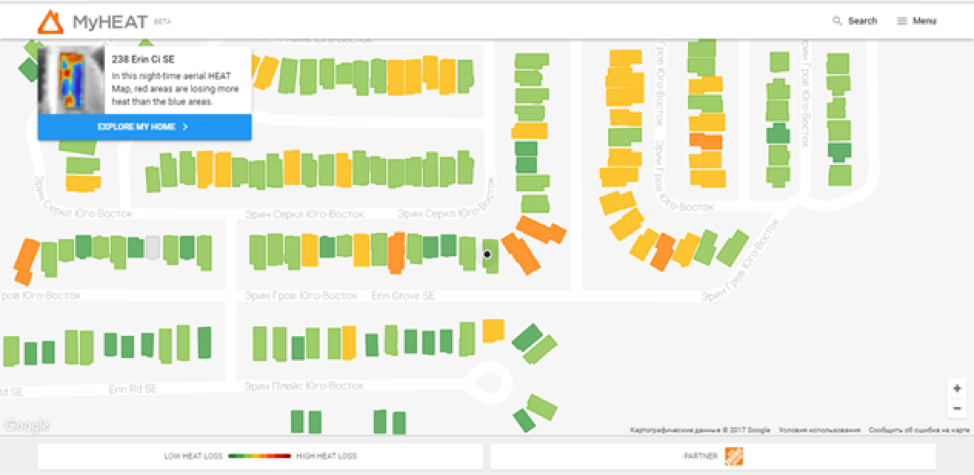
\includegraphics[width=0.9\textwidth]{images/screens/0_myheat.png}
      \caption{Внешний вид интерфейса системы MyHEAT}
      \label{screens:myheat}
    \end{figure}

\subsection{National Heat Map}

\par
	\textbf{National Heat Map} - разработка Центра по устойчивой энергетике (CSE) в Великобритании. Этот проект существует с 2010 года, данные в нём постоянно обновляются [*]. NHM позволяет получать данные по адресам зданий, в открытом доступе предоставляет интерактивную тепловую карту с выбором различных слоёв по категориям зданий (производственные, коммерческие и жилые). Эти слои представляют собой цветные изображения областей по уровням тепловыделения.

 	Данные о распределении тепла в конкретных зданиях предоставляются административным органам, а также организациям, имеющим специальную лицензию. Отличительная особенность данной системы - проработанный веб-интерфейс, который позволяет рассматривать карту по разным слоям одновременно, выделять интересующие области. Имеется возможность вывода результатов статистических расчётов по выбранной области в различных форматах (табличные, такие как \texttt{CSV}, диаграммы и графики). [*] Такое решение подходит для случаев, когда нужен охват территории в масштабе целого континента. Однако оно не позволяет увидеть оценки для конкретных зданий в открытом виде, предоставляя лишь усреднённые показатели для комплексов зданий или отдельных улиц, районов и т. п.

 	\begin{figure}[h!]
      \centering
      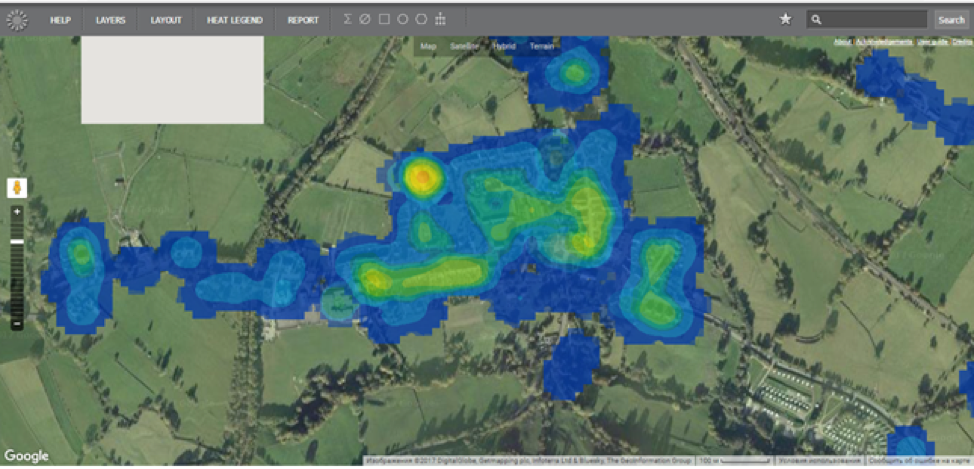
\includegraphics[width=0.9\textwidth]{images/screens/1_nhm.png}
      \caption{Внешний вид интерфейса системы National Heat Map}
      \label{screens:nhm}
    \end{figure}

\subsection{HEAT}

\par
	\textbf{HEAT} - веб-ориентированная система анализа потерь тепла, использующая тепловые аэроснимки. Используются стандарты \texttt{OGC} (Open Geospatial Consortium) для геопространственных сервисов.[*], картографический сервис \texttt{Google Maps} с возможностью выбора слоя тепловых утечек. Слой представляет из себя совокупность зданий, каждое из которых окрашено в соответствии с присвоенным ему одним из десяти классов энергетической эффективности, основанных на средней температуре крыш всех зданий. Система предоставляет такую информацию, как:

	\begin{itemize}
		\item минимальная и средняя температуры поверхности крыши выбранного здания;
		\item три наиболее горячие точки на поверхности крыши;
		\item суточную стоимость отопления дома и количество выделяющегося при этом углекислого газа в зависимости от вида топлива (газ/уголь/возобновляемые источники энергии);
		\item количество топлива, его стоимость и величина выделяемого углекислого газа, которые можно сократить при условии уменьшения температуры крыши до минимальной.
	\end{itemize}

	Важной особенностью сервиса является использование решений Geographic Object Based Image Analysis (\texttt{GEOBIA}), позволяющих в автоматическом или полуавтоматическом режиме генерировать готовые к внедрению в ГИС полигоны домов, анализируя непосредственно тепловые аэроснимки, а не используя имеющиеся городские кадастровые данные. Это играет существенную роль, когда кадастровые данные недоступны, и позволяет получить доступ к информации через веб-страницу в течение недели после сбора данных.

	\begin{figure}[h!]
      \centering
      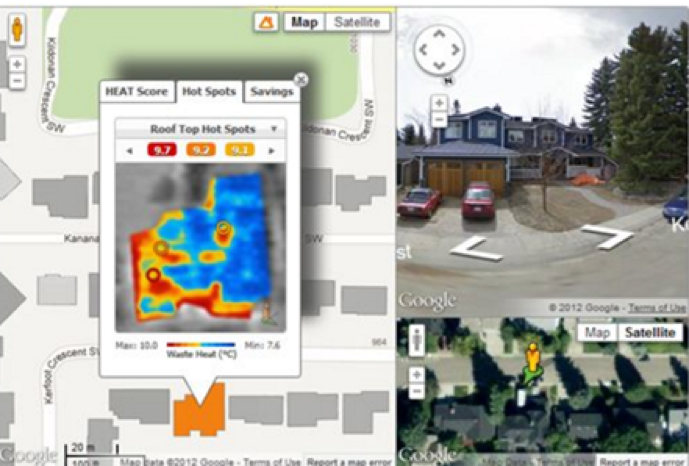
\includegraphics[width=0.9\textwidth]{images/screens/2_heat.png}
      \caption{Внешний вид интерфейса системы HEAT}
      \label{screens:heat}
    \end{figure}

\subsection{blomURBEX}

\par
	\textbf{blomURBEX} - разработка норвежской компании Blom. Представляет из себя веб-сервис, предоставляющий доступ к карте, на которую добавлены слой информации об утечках тепла и оценка, присваиваемая теплоэнергетической эффективности здания. Можно производить поиск по адресу, также предусмотрена навигация по карте. Есть возможность нанесения на карту дополнительных графической объектов и текста, сохранения результатов в файл.

\subsection{Jersey Heat Loss Map}

\par
	Интерактивная карта, разработанная службой энергоэффективности (EES) острова Джерси, ориентирована не только на городские коммунальные службы, но и на самих владельцев домов, позволяя им увидеть оценку результатов тепловизионного анализа по установленной шкале уровней тепловых утечек. Сами здания на карте представлены прямоугольниками разных цветов, соответствующих уровням этой шкалы. По каждому объекту можно получить такую информацию, как тип здания, индекс тепловых потерь и его текстовое описание. Из недостатков данной системой существенными являются отсутствие возможности увидеть изображения распределения тепла и получить статистику в произвольном масштабе.

\subsection{Оценка аналогов}

\par

	Для сравнения аналогов были выбраны критерии, по которым будет производиться оценка. Кортежная модель оценки аналогов имеет вид:

	\begin{center}
		ОА=<О(УФ), О(РТ), О(РЭ), О(ГП), О(КС), О(СР), О(ПЗ); R>, 
	\end{center} 

	где ОА - оценка аналога,

	О(УФ) - оценка учета факторов,

	О(РТ) - оценка предоставления информации о распределении температур,

	О(РЭ) - оценка расчета энергии,

	О(ГП) - оценка генерации полигонов,

	О(КС) - оценка количества слоев,

	О(СР) - оценка выдачи статистических расчетов,

	О(ПЗ) - оценка поиска зданий,

	R - матрица связи.

	\textbf{Учет факторов}. Первый критерий - учет факторов - подразумевает “выравнивание” результатов с учетом изменения микроклимата от одного здания к другому, учет материалов крыш, использование алгоритмов повышения достоверности информации. Данный критерий оценивается следующим образом:

	\begin{center}
		\begin{equation*}
			I_\textup{УФ} = 
	 		\begin{cases}
	   			1, &\text{если учитывается микроклимат и материал крыши}\\
	   			0.5, &\text{если используются статистические данные} \\
	   			0, &\text{если дополнительные факторы не учитываются}
	 		\end{cases}
		\end{equation*}
	\end{center}

	\textbf{Распределение температур}. Критерий оценивается в зависимости от того, предоставляет ли выбранный аналог информацию о распределении температур по поверхности крыш зданий или нет:

	\begin{center}
		\begin{equation*}
			I_\textup{РТ} = 
	 		\begin{cases}
	   			1, &\text{если система предоставляет информацию о распределении температуры по обследуемой поверхности здания}\\
	   			0, &\text{если система не предоставляет такую информацию}
	 		\end{cases}
		\end{equation*}
	\end{center}

	\textbf{Расчет энергии}. Критерий оценивается в зависимости от предоставления системой информации о количестве энергии, затрачиваемой на отопление дома:

	\begin{center}
		\begin{equation*}
			I_\textup{РЭ} = 
	 		\begin{cases}
	   			1, &\text{если система предоставляет информацию о количестве энергии, затрачиваемой на отпление дома}\\
	   			0, &\text{если система не предоставляет такую информацию}
	 		\end{cases}
		\end{equation*}
	\end{center}

	\textbf{Генерация полигонов}. Оценка производится на основе возможности системы создавать полигоны зданий, используя распознавание объектов и не прибегая к кадастровой информации.

	\begin{center}
		\begin{equation*}
			I_\textup{ГП} = 
	 		\begin{cases}
	   			1, &\text{если система генерирует полигоны}\\
	   			0, &\text{если система не генерирует полигоны}
	 		\end{cases}
		\end{equation*}
	\end{center}

	\textbf{Количество доступных слоев}. При отображении карты на нее могут накладываться слои с различной вспомогательной информацией, статистическими данными и выбранными фильтрами. Оценка этого критерия производится следующим образом:

	\begin{center}
		\begin{equation*}
			I_\textup{КС} = 
	 		\begin{cases}
	   			1, &\text{если имеется три и более слоёв}\\
	   			0.5, &\text{если имеется два слоя} \\
	   			0, &\text{если имеется один слой}
	 		\end{cases}
		\end{equation*}
	\end{center}

	\textbf{Статистические расчеты}. Оценка этого критерия производится в зависимости от возможности предоставления системой статистических расчетов:

	\begin{center}
		\begin{equation*}
			I_\textup{СР} = 
	 		\begin{cases}
	   			1, &\text{если система предоставляет статистические расчёты по выбранной территории с учётом параметров, характеризующих здания и специфику местности}\\
	   			0, &\text{если система не предоставляет такую информацию}
	 		\end{cases}
		\end{equation*}
	\end{center}

	\textbf{Поиск зданий}. Оценка критерия производится следующим образом:

	\begin{center}
		\begin{equation*}
			I_\textup{СР} = 
	 		\begin{cases}
	   			1, &\text{если предусмотрена возможность поиска зданий по адресу}\\
	   			0, &\text{если такая возможность не предусмотрена}
	 		\end{cases}
		\end{equation*}
	\end{center}

	Оценка аналогов будет производиться по следующей формуле:

	\begin{center}
		ОА = О(УФ)$\cdot\alpha$(УФ)+О(РТ)$\cdot\alpha$(РТ)+О(РЭ)$\cdot\alpha$(РЭ)+

		+О(ГП)$\cdot\alpha$(ГП)+О(КС)$\cdot\alpha$(КС)+О(СР)$\cdot\alpha$(СР)+О(ПЗ)$\cdot\alpha$(ПЗ),
	\end{center}

	где $\sum\limits_{i=1}^{n}{\alpha_{i}} = 1$, $\alpha_{i}$ --- весовой коэффициент $i$-го критерия.

\par
	\textbf{Определение весовых коэффициентов критериев}.

	При методе попарных сравнений используется шкала словесных определений уровня важности, где каждому определению ставится в соответствие число (таблица \ref{table:scale})

	\begin{table}[h!]
		\begin{center}
			\caption{Шкала уровней важности}
			\begin{tabular}{ | p{0.6\textwidth} | p{0.3\textwidth} | }
				\hline
				Уровень важности & Количественное значение \\
				\hline
				Равная важность & 1 \\
				\hline
				Промежуточное значение между равенством и слабым превосходством & 2 \\
				\hline
				Умеренное превосходство & 3 \\
				\hline
				Промежуточное значение между слабым и сильным превосходством & 4 \\
				\hline
				Существенное или сильное превосходство & 5 \\
				\hline
				Промежуточное значение между сильным и значительным превосходством & 6 \\
				\hline
				Значительное (большое) превосходство & 7 \\
				\hline
				Промежуточное значение между значительным и абсолютным превосходством & 8 \\
				\hline
				Абсолютное превосходство & 9 \\
				\hline
			\end{tabular}
			\label{table:scale}
		\end{center}
	\end{table}

	\pagebreak

	Оценка аналогов производилась с использованием методики Томаса Саати. На таблице \ref{table:est} представлена матрица попарного сравнения критериев.

	\pagebreak

	\begin{table}
		\begin{center}
			\caption{Оценка весовых коэффициентов критериев}
			\begin{tabular}{ | p{0.3\textwidth} | l | l | l | l | l | l | l | c | c | }	
				\hline
				   & УФ & РТ & РЭ & ГП & КС & СР & ПЗ & $\Sigma$ & $\alpha$ \\
				\hline
				УФ &1   &2   &3   &4   &5   &6   &8   &29.00 &0.26 \\
				\hline
				РТ &1/2 &1   &2   &4   &6   &7   &9   &29.50 &0.26 \\
				\hline
				РЭ &1/3 &1/2 &1   &3   &5   &5   &7   &21.83 &0.19 \\
				\hline
				ГП &1/4 &1/4 &1/3 &1 &  3   &3   &6   &13.83 &0.12 \\
				\hline
				КС &1/5 &1/6 &1/5 &1/3 &1   &2   &5   &8.90  &0.08 \\
				\hline
				СР &1/6 &1/7 &1/5 &1/3 &1/2 &1   &4   &6.34  &0.06 \\
				\hline
				ПЗ &1/8 &1/9 &1/7 &1/6 &1/5 &1/4 &1   &2.00  &0.02 \\
				\hline
				ЭР &1/9 &1/9 &1/8 &1/7 &1/6 &1/6 &1/2 &1.32  &0.01 \\
				\hline 
				\multicolumn{8}{|c|}{$\Sigma\Sigma$}           &112.73 &1   \\
				\hline
			\end{tabular}
			\label{table:est}
		\end{center}
	\end{table}

	В таблице \ref{table:critval} приведены оценки аналогов по выбранным критериям.

	\begin{table}[h!]
		\begin{center}
			\caption{Показатели критериев аналогов}
			\begin{tabular}{ | p{0.43\textwidth} | l | l | l | l | l | l | l | l | }	
				\hline
				  	                        &УФ  &РТ &РЭ &ГП &КС  &СР &ПЗ &ЭР \\
				\hline
					Jersey Heat Loss Map 	&0   &0  &0  &0  &0   &0  &1 &0 \\
				\hline
					HEAT 					&1   &1  &1  &1  &0,5 &0  &0 &0 \\
				\hline
					MyHEAT 					&1   &1  &1  &1  &0   &0  &1 &0 \\
				\hline
					BlomURBEX 				&0   &0  &0  &0  &0,5 &0  &1 &1 \\
				\hline
					National Heat Map 		&0.5 &0  &1  &0  &1   &1  &1 &1 \\
				\hline
			\end{tabular}
			\label{table:critval}
		\end{center}
	\end{table}

	\pagebreak

	Взвешенные оценки аналогов представлены в таблице \ref{table:weightedest}.

	\begin{table}[h!]
		\begin{center}
			\caption{Оценки аналогов по критериям}
			\begin{tabular}{ | l | l | l | l | l | l | l | l | l | l | }	
				\hline
				 	&УФ &РТ &РЭ &ГП &КС &СР &ПЗ &ЭР &$\alpha$\\
				\hline
					&0.26 &0.26 &0.19 &0.12 &0.08 &0.06 &0.02 &0.01 &1.00 \\
				\hline
					Jersey Heat Loss Map &0 &0 &0 &0 &0 &0 &0.02 &0 &0.02 \\
				\hline
					HEAT &0.26 &0.26 &0.19 &0.12 &0,04 &0 &0 &0 &0.87 \\
				\hline
					MyHEAT &0.26 &0.26 &0.19 &0.12 &0 &0 &0.02 &0 &0.85 \\
				\hline
					BlomURBEX &0 &0 &0 &0 &0,04 &0 &0.02 &0.01 &0.07 \\
				\hline
					National Heat Map &0.13 &0 &0.19 &0 &0.08 &0.06 &0.02 &0.01 &0.49 \\
				\hline
			\end{tabular}
			\label{table:weightedest}
		\end{center}
	\end{table}

	Наиболее высокую оценку получил аналог HEAT, целесообразно рассматривать его в качестве прототипа.

\section{Критика прототипа}

\par
	В результате оценки аналогов наилучший результат получил система HEAT Университета Калгари, Канада. Основные ее преимущества - использование алгоритмов повышения достоверности результатов, автоматическая генерация полигонов зданий.
	
	Существенный недостаток системы HEAT --- отсутствие возможности работы с пользовательскими данными. Не предусмотрена функция загрузки снимков и вспомогательных данных с пользовательских устройств (в частности, со смартфонов) и их последующая обработка. Доработка этих возможностей позволит наполнить систему более полной и актуальной информацией в соответствии с принципами \texttt{VGI}. 


\section{Аналоги по подсистеме}

\textcolor{red}{Раздел в доработке.}

\section{Уточнение целей и задач}

\par

	Глобальная цель работы --- повышение достоверности результатов обследования жилых зданий с целью выявления утечек тепла.

	Локальной целью является разработка программного интерфейса (\texttt{API}), позволяющего подключать к системе приложения сторонних разработчиков на различных устройствах.

	Задачи, которые необходимо решить для достижения поставленной цели:

	\begin{itemize}
		\item Выполнить аналитический обзор имеющихся в мире информационных систем, выполняющих задачу контроля тепловой энергоэффективности;
		\item Провести анализ современных технологий, применяющихся для получения исходных данных, циркулирующих в этих системах;
		\item Обнаружить среди обозреваемых систем и технологий наиболее совершенные с точки зрения поставленной в данной работе цели и выделить прототип разрабатываемой системы;
		\item Разработать пакет моделей на создание улучшенной информационной системы;
		\item Выполнить внешнее и внутреннее проектирование искомой системы;
		\item Реализовать программное решение искомой системы.
	\end{itemize}

\section{Результаты и выводы по главе 1}

\par

	Проведён поиск информации об используемых решениях в области систем контроля тепловой энергоэффективности зданий. Выполнен обзор литературных источников и существующих аналогов таких систем, сформулировано их общее описание. Среди аналогов на основе оценки наиболее существенных факторов выявлен прототип. На основании критики предложена доработка прототипа. Определены цели и задачи данной работы.


